\documentclass[11pt]{article}
\usepackage[utf8]{inputenc}
\usepackage{fullpage}
\usepackage{authblk}
\usepackage{url}
\usepackage{physics}
\usepackage{amsmath}
\usepackage{amssymb}
\usepackage{float}
\usepackage{tikz}
\usepackage{hyperref}
\usepackage{verbatim}
\usepackage[font=small,labelfont=bf, skip=1pt,center]{caption}
\DeclareMathOperator*{\minimize}{minimize}
\usepackage{bm}
\usepackage{booktabs}
\usepackage{tabularx}

\newcommand{\normnew}[2]{\left \lVert #1 \right \rVert_{#2}}

\counterwithout{figure}{section}


%\title{AA203 Report Template}
\title{AA203 Project: Pesticide use optimization \\ Follow-up Report}

\author{Stuart Johnson}
\affil{stujohn@stanford.edu, stuart.g.johnson@gmail.com}

\date{\today}

\begin{document}

\maketitle

\begin{abstract}
Optimizing spatio-temporal pesticide application during the growing season can have a significant impact on pesticide cost and the quantity of pesticides being applied and released into the environment. We apply optimal control techniques to a synthetic crop field and demonstrate potentially significant impact in reducing pesticide usage. The magnitude of the impact depends heavily on the details of the crop ecosystem. In this follow-up report, more care is taken in making sure the calculations converge to a given tolerance via a combination of an adaptive trust region implementation and spatial grid refinement.
\end{abstract}

\section{Introduction}
When managing a field of crops, one of the challenges is protecting the crop from consumption by pests - in particular, competing with insects for harvestable food. While there are organic practices for farming, these do not necessarily obviate the need for pesticides. In any case, it is of interest to optimize pesticide application in time and space, both from an economic and ecological health perspective. This project aims to quantify optimized pesticide application in several cases by applying the methods of optimal control. In particular, to quantify the impact of pesticide timing and spatial application in precision agriculture settings relative to exhaustive techniques - like aerial spraying of the entire field.

\section{Related Work}
Papers investigating complex (or otherwise) optimal controls in 2D for agricultural purposes are not abundant. However, there are numerous papers investigating controls for more complex combinations of pests and plants or even for irrigation control - in time and - at most - a single spatial dimension. Examples are given in \cite{R1} and \cite{R2}. Since various agricultural practices involve spatial patterns of ecosystem management - like crop rotation, for example \cite{R3}, it seems possible that the literature is missing some possible refinement of agricultural ecosystem control practices by not considering 2D scenarios.

\section{Problem Statement}
Let us suppose we are managing a crop in a square field. This crop is planted and grown for a number of months and then harvested essentially all at once (an example would be corn).

A common approach to modelling ecological problems is the reaction-diffusion (RD) equation. This allows us to model the spatial movement of chemical or biological actors and also model the life cycle and interaction of the same actors. For this project, we adopt a version of the RD equation which only models the pest as obeying spatial diffusion. The RD PDE for our crops is:

\begin{align}
	\label{eqn:pde}
	\dv{c(x,y,t)}{t} &= -k_{cp} p c + k_c \left( 1 - \frac{c}{K_c} \right) c \nonumber \\ 
	\dv{p(x,y,t)}{t} &= d_p \laplacian{p} - k_{pw} w p + k_{pc} c p - k_p p \\
	\dv{w(x,y,t)}{t} &= u - k_w w \nonumber
\end{align}

where, defined on the domain $\Omega$ of the crop field:

\begin{itemize}
\setlength\itemsep{-1pt}
\item $c(x,y,t)$ crop density ; \textbf{state}
\item $p(x,y,t)$ pest density ; \textbf{state}
\item $w(x,y,t)$ pesticide density ; \textbf{state}
\item $u(x,y,t)$ pesticide application rate ; \textbf{control}
\item $k_{cp} = 0.2$ rate of crop consumption by pest
\item $k_c = 0.1$ rate of crop growth
\item $K_c = 1.0$ carrying capacity (density) of field for crop
\item $d_p = 0.05 - 0.40$ diffusion coefficient of pests
\item $k_{pw} = 0.3$ rate of pest death by pesticide
\item $k_{pc} = 0.2$ rate of pest growth (requires crop)
\item $k_p = 0.025$ rate of pest death
\item $k_w = 0.2$ rate of pesticide decay - as a toxin \textit{and} as a disagreeable food additive \cite{R4}
\end{itemize}

subject to initial conditions:

\begin{itemize}
\setlength\itemsep{-1pt}
\item $c(x,y,0) = 0.5$ initial crop density ; \textbf{state}
\item $p(x,y,0) = 0.0$ initial pest density ; \textbf{state}
\item $w(x,y,0) = 0.0$ initial pesticide density ; \textbf{state}
\end{itemize}

and boundary conditions defined on the crop field boundary $\partial\Omega$:

\begin{itemize}
\setlength\itemsep{-1pt}
\item $p = 0$ homogeneous Dirichlet pest density at the boundary
\item or
\item $\nabla p(x,y,t) \cdot \hat{n} = b_p(x,y,t)$ inhomogeneous Neumann normal pest flux at the boundary
\end{itemize}

[Important note/Disclaimer: the parameters of this RD model are not necessarily indicative of actual parameters to be encountered in an any actual field of crops. Parameters were varied and sampled in such a way to yield interesting model behavior and investigate the numerical techniques involved.]

We model crop density limits via "logistic" growth in the term $k_c \left( 1 - \frac{c}{K_c} \right) c$. This limits the equilibrium crop density to $K_c$. This PDE exhibits a number of interesting growth/consumption patterns - like waves of pest density moving in response to crop consumption and pest diffusion.

Initial and boundary conditions are used to specify the nature of a pest attack during the growing season. For the purposes of the analysis below, we will assume a constant in time, spatially variable flux of pests into our crop field. This flux will specifically model a concentration of flux coming from the southeast (see Figure 4 in the Appendix) - representative of being close to a natural reservoir, for example, and some level of background flux elsewhere. The nature of the pest attack is a very important factor in the analysis.

Our problem is to optimize the spatio-temporal application of pesticide in order to minimize the impact of pests and pesticide on the crop at harvest time. This is implemented via minimizing a combination of (see also the section on $P$ and $Q$ cost matrices below) the following both during the growing season and at harvest time:

\begin{itemize}
\setlength\itemsep{-1pt}
\item Active pesticide density across the field
\item Pest density across the field
\item Crop yield loss across the field
\end{itemize}

These are conflicting goals - for example, pesticide application increases crop yield but also contaminates the harvested crop. The behavior of the PDE is strongly dependent on the parameters and initial and boundary conditions used to model the crop/pest ecosystem and the pest attack. As noted above, this model has not been calibrated or tuned to represent a realistic scenario.

\section{Approach}

The transcribed, constrained optimal control problem corresponding to the problem statement is:

\begin{align}
\label{eqn:ocp}
\minimize_{s,u} J=& \sum_{k=0}^{N-1} \left( (s_k - s_{goal})^T Q (s_k - s_{goal}) + u_k^T R u_k \right) \\
	     & \qquad \qquad  + (s_N - s_{goal})^T P (s_N - s_{goal}) \nonumber  \\
\text{subject to} \qquad s_0 &= \bar{s}_0 \nonumber \\
s_{k+1} &= f_d(s_k, u_k), \forall k \in \{ 0,1,\dots , N-1 \} \nonumber \\
u_k &\geq 0, \forall k \in \{ 0,1,\dots, N-1\} \nonumber \\	   
u_k &\leq u_{max}, \forall k \in \{ 0,1,\dots, N-1 \} \nonumber	     
\end{align}
 
where (see also the Experiments section):

\begin{itemize}
\setlength\itemsep{-1pt}
\item $J$ is the objective to be minimized
\item $k \in \{0, \dots N-1\}$ is the discrete time index, where $N = T/dt$
\item $T$ is the harvest time, and $dt$ is the discrete time step
\item $f_d$ is the discrete time, locally linearized evolution of state (from equation \ref{eqn:pde})
\item $s_k \in \mathbb{R}^{3n^2}$
\item $u_k \in \mathbb{R}^{n^2}$ for full control, or:
\item $u_k \in \mathbb{R}^{1}$ for aerial spraying control, or:
\item $\bar{s}_0$ is $c = C_0$, $p = 0$, $w = 0$
\item $C_0$ is the spatially constant crop density at time $0$
\item $s_{goal}$ is $c = C_N$, $p = 0$, $w = 0$
\item $C_N$ is crop density at harvest time $T = N dt$ assuming no pest damage (following the crop growth rate)
\end{itemize}

The cost matrices need to weight the deviation of $c$, $p$ and $w$ from their goal states in such a way to result in a desired trade-off between these costs at harvest time ($P$) and during the growing season ($Q$). After some numerical experimentation, we use the following weights for these diagonal matrices. The total weight for each section of the matrix is the product of the overall factor and the factor for $c$, $p$, $w$ and $u$.

\begin{center}
	\begin{tabular}{ | c | c | c | c | c | c | }
	\hline
    cost matrix & overall & $c$ & $p$ & $w$ & $u$ \\
    \hline
    P & 100 & 1 & 10 & .01 & 0 \\
    \hline
    Q & 0.1 & 1 & 10 & .01 & 0 \\
    \hline
    R & .001* & 0 & 0 & 0 & 1 \\
    \hline
    \end{tabular}
    \captionof{table}{Cost matrix weighting. *Note that R has an additional factor for aerial spraying.}
\end{center}

For aerial spraying, where $u_k \in \mathbb{R}^{1}$, we additionally weight $R$ by $n^2$ (where the spatial grid is $n \times n$) to make the penalty on the control across the field the same as it would be for a comparable spot spraying optimal control scenario.

After spatial discretization of the crop field into $n \times n$ equally spaced points (with a point on the boundaries), the PDE in equation \ref{eqn:pde} above is converted into a coupled system of ODEs. The Laplacian becomes a (quite sparse, block-diagonal-dominant) matrix $L$. For the purposes of this project, the Laplacian has been discretized for both 1) Dirichlet and 2) Neumann boundary conditions \cite{R5}. When homogenous (0), these boundary conditions correspond, respectively, to 1) no pest at the field boundaries or 2) a boundary impermeable to pests. As mentioned above, we will be simulating a time-constant, spatially varying boundary-normal flux of pests into our field via inhomogenous Neumann boundary conditions. Equation 1 becomes:

\begin{align}
\dot{\bm{c}} &= -k_{cp} \bm{p} \odot \bm{c} + k_c \left( 1 - \frac{\bm{c}}{K_c} \right) \odot \bm{c} \nonumber \\ 
\dot{\bm{p}} &= d_p \frac{L}{h^2} \bm{p} + \frac{\bm{b}_p}{h} - k_{pw} \bm{w} \odot \bm{p} + k_{pc} \bm{c} \odot \bm{p} - k_p \bm{p} \\
\dot{\bm{w}} &= \bm{u} - k_w \bm{w} \nonumber
\end{align}

where

\begin{itemize}
\setlength\itemsep{-1pt}
\item $\odot$ is the element-wise product
\item $L$ is the finite difference matrix for Neumann boundary conditions
\item $\bm{b}_p$ is the boundary flux of pests, defined at the boundary points
\item $n$ is the spatial grid resolution (the grid is $n \times n$)
\item $h = D / (n-1)$ is the grid cell size
\item $D$ is the spatial extent of the crop field ($D \times D$) in each dimension
\end{itemize}

The $h^2$ factor has not been included in $L$ to make it clear which terms depend explicitly on the grid resolution or the spatial extent of the crop field $D$. A clear and explicit discussion of the Laplacian finite difference matrix can be found in \cite{R5}. Also, as we will be refining the grid to accelerate convergence of SCP (Sequential Convex Programming), the correct dependence on $h$ is essential.

SCP (Sequential Convex Programming) with a trust region approach is applied to this optimal control problem (equation \ref{eqn:ocp}). The linearized $f_d$ is computed by fourth order Runge-Kutta integration with linearization provided by the \texttt{JAX} computation of the Jacobian. \texttt{CVXPY} is used to compute the optimal solution. While it was found that one might be lucky with a fixed trust region size and some parameters of the PDE, generally speaking a robust SCP solution was found to require an adaptive trust region approach. Otherwise the solution would, at best, be slow to converge.

A minimal implementation of an adaptive trust region was used. The trust region constrains the update in the state $s$ and control $u$ at each iteration $i$ of SCP such that:

\begin{align}
\normnew{u^{(i)} - u^{(i-1)}}{\infty} &\leq \rho \nonumber \\
\normnew{s^{(i)} - s^{(i-1)}}{\infty} &\leq \rho \nonumber 
\end{align}

where we have boldly conflated all components (variously scaled, no doubt!) of the solution such that they can be usefully measured with a single distance $\rho$. As SCP progresses - or even on the first iteration, one needs a mechanism to check and adjust $\rho$.

The adaptive trust region utilized here is based on discussion in \cite{R6}, equations 1.4-1.6. In particular, let:

\begin{align}
r_{i} &= \frac{J(s^{(i)}) - J(s^{(i+1)})}{\hat{J}(s^{(i)}) - \hat{J}(s^{(i+1)})}
\end{align}

where $\hat{J}$ is the value of the objective based on the locally linearized PDE (for this step of SCP), and $J$ is the objective based on integration of the full nonlinear PDE using the approximation of $u$ from the $ith$ step of SCP. Equivalently:

\begin{align}
r_i &:= \frac{\text{Actual reduction in J}}{\text{Predicted reduction in J}}
\end{align}

Subsequent to this evalation of $r$ at each step of SCP, we then take action to 1) accept or deny the approximate solution, and 2) expand, contract, or keep the current trust region $\rho$:

\begin{align}
\text{if } r_i &\geq \eta_1 : \text{accept the update of } \{s,u\} \nonumber \\
\text{if } r_i &> \eta_2 : \rho = \max\left(\beta \rho, \rho_{min}\right) \nonumber \\
\text{if } r_i &< \eta_1 : \rho = \max\left(\rho / \beta, \rho_{min}\right) \nonumber
\end{align}

where we now have some hyperparameters to determine. Some numerical experimentation settled on:

\begin{itemize}
\setlength\itemsep{-1pt}
\item $\rho_{init} = 0.5$
\item $\rho_{min} = 0.01$
\item $\beta = 2$
\item $\rho_1 = 0.5$
\item $\rho_2 = 0.99$
\end{itemize}

This adaptive trust region algorithm is implemented in \texttt{scp\_pest.solve\_scp\_plus()}.

There are two other general considerations for the accuracy of approximation of the PDE. One is the time increment $dt$, and the other is the spatial resolution $n$. Via numerical experimentation, $dt = 0.05$ was found to result in stable results across the PDE parameter ranges (specifically $d_p = 0.05 - 0.4$) used in the numerical experiments below. Some simulation of the PDE suggests that (for zero control and $d_p = 0.25$) the solution improves significantly out to $n = 24$ (where relative errors are around $1\%$):

\begin{center}
\begin{tabular}{rrrrr}
\toprule
$n_{ref}$ & n & $\| c_{ref} \|_{\infty}$ & $\| c-c_{ref} \|_{\infty}$ & $\frac{\| c-c_{ref} \|_{\infty}}{\| c_{ref} \|_{\infty}}$ \\
\midrule
32 & 32 & 0.619 & 0.000 & 0.000 \\
32 & 28 & 0.619 & 0.003 & 0.005 \\
32 & 24 & 0.619 & 0.007 & 0.012 \\
32 & 20 & 0.619 & 0.015 & 0.024 \\
32 & 16 & 0.619 & 0.025 & 0.040 \\
32 & 12 & 0.619 & 0.036 & 0.058 \\
32 & 8 & 0.619 & 0.067 & 0.108 \\
32 & 4 & 0.619 & 0.160 & 0.258 \\
\bottomrule
\end{tabular}
\end{center}

\begin{center}
\begin{tabular}{rrrrr}
\toprule
$n_{ref}$ & n & $\| p_{ref} \|_{\infty}$ & $\| p-p_{ref} \|_{\infty}$ & $\frac{\| p-p_{ref} \|_{\infty}}{\| p_{ref} \|_{\infty}}$ \\
\midrule
32 & 32 & 1.173 & 0.000 & 0.000 \\
32 & 28 & 1.173 & 0.009 & 0.008 \\
32 & 24 & 1.173 & 0.020 & 0.017 \\
32 & 20 & 1.173 & 0.042 & 0.036 \\
32 & 16 & 1.173 & 0.071 & 0.061 \\
32 & 12 & 1.173 & 0.099 & 0.084 \\
32 & 8 & 1.173 & 0.178 & 0.152 \\
32 & 4 & 1.173 & 0.385 & 0.328 \\
\bottomrule
\end{tabular}
\end{center}

In both these tables, we have used the \texttt{scipy odeint} solver to arrive at accurate solutions at each level of spatial discretization. This suggests that we need to refine the spatial grid for accurate solutions (see below). Code for these convergence tables can be found in \texttt{test\_convergence.py}.

As a practical computational matter, SCP with \texttt{JAX/CVXPY} is reasonably performant only to modest grid sizes. Running SCP using the \texttt{ECOS} solver, $5 \times 5$ discretizations are relatively tractable and converge to results in a few minutes. $7 \times 7$ discretizations require hours to converge. A critical step here is using the \texttt{MOSEK} solver - which, unfortunately, requires a license. The \texttt{MOSEK} solver allows for grids out to at least $16 \times 16$ discretizations - which will run in several minutes per SCP iteration (see the experiments section below). When running $20 \times 20$ discretizations, it would appear that the solver exhausts system memory (32 GB in this case). It is not clear if there is a way to alleviate the memory situation by modifying code. More memory is certainly an option - suggesting running on cloud resources. Note that an $n=20$ SCP problem has a state space of dimension 1200. Results shown below use the \texttt{MOSEK} solver.

While convergence is shown in detail in the appendix, the refinement of the spatial solution is included in the SCP iterations - as an outer loop. The grid refinement is controlled via a schedule, and the final change in relative error of the objective $J$ is reported. Prospective solutions at higher resolutions are obtained by linear interpolation of the spatial state and control fields using \texttt{opencv.resize()}.  This is implemented in \texttt{scp\_pest.do\_scp\_plus\_plus()}. Interpolating the state fields when proceeding to higher spatial resolution does not work as well as interpolating the control field, then re-integrating the ODE to obtain a starting state solution for an iteration of the SCP outer loop.

Finally, convergence is monitored via relative error in the objective $J$. As noted above, the optimal $J$ is non-zero: the objective combines several conflicting goals. It is quite likely there are better ways to measure (relative) error and convergence - such as the total pesticide dose over time or some other combination of the solution components over the growing season.

\section{(Numerical) Experiments}

We investigate the impact of a spatio-temporal approach to optimizing pesticide application as opposed to spatially constant, but time varying application. The latter would represent, for example, aerial spraying over the entire field. In both cases we assume a persistent pest hazard from adjacent land over the growing season. We compare pesticide quantities applied for two cases (Exp 1 and 2).

\begin{itemize}
	\setlength\itemsep{-1pt}
	\item Exp 1: Aerial spraying: spatially uniform application of pesticide (aerial spraying), with the time dependence to be found by optimal control. Compute total pesticide quantity applied. $d_p$, the pesticide diffusion constant, is varied from $.05 - 0.4$.
	\item Exp 2: Spot spraying: optimal time and spatial pattern of pesticide application rate $u$ to be found via optimal control methods. Compute total pesticide quantity applied. $d_p$, the pesticide diffusion constant, is varied from $.05 - 0.4$.
\end{itemize}

As opposed to the previous report (\texttt{reports/final\_report.pdf}), we do not show results for no control (0 pesticide rate). We compare results for the re-simulated growing season using the optimal controls $u$ computed by SCP for each condition - although the difference in state space between the re-simulated and state space resulted returned by SCP were not significant.

\subsection{Exp 1: Aerial Spraying}

Aerial spraying is defined by spatially constant control - or the same spraying rate across the whole field. We find the optimal time trajectory of this control via SCP. 

For Exp 1, the optimal control solutions (figure \ref{fig: aerialslow} and figure \ref{fig: aerialfast} and figure 5 in the Appendix) show a mildly oscillatory control pattern, with a rise in pesticide application rate in the middle of the growing season. The optimal control problem penalizes the density of active pesticide at harvest time, so early applications of pesticide are preferred. Generally speaking, when we interchange the relative weightings of the $P$ and $Q$ cost matrices (so the terminal cost is reduced), the optimal control is non-zero much later in the growing season.

\begin{minipage}{\textwidth}
	\begin{center}
		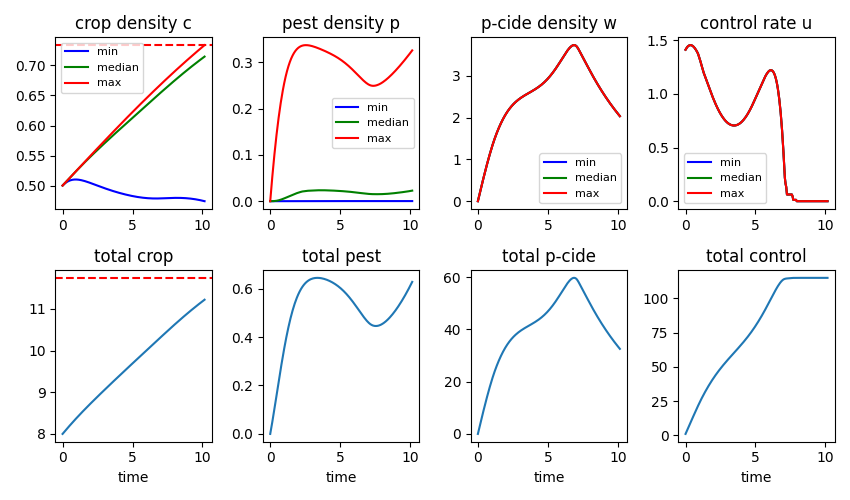
\includegraphics[width=0.8\linewidth]{../resim_240718-021040/time.png}
		\captionof{figure}{Pest attack scenario with aerial spraying control. In the top row, min, median and max curves capture spatial variability. Slow pest diffusion: $d_p = 0.05$.}
		\label{fig: aerialslow}
	\end{center}
\end{minipage}

\begin{minipage}{\textwidth}
	\begin{center}		
		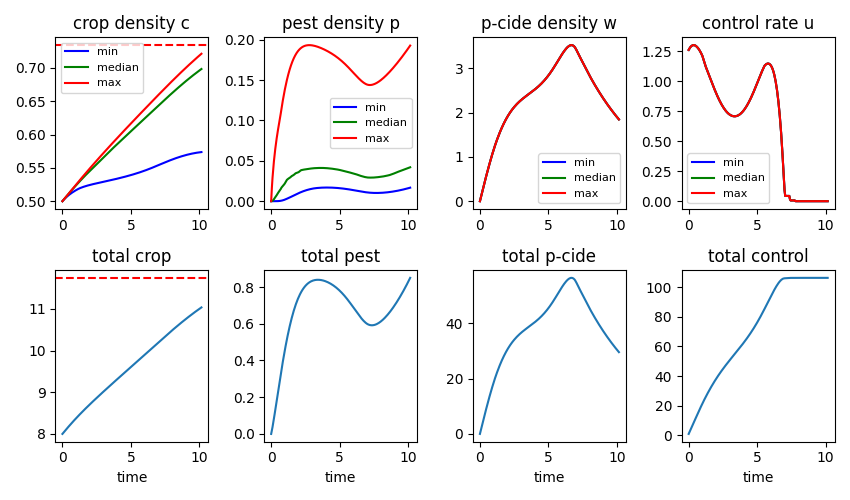
\includegraphics[width=0.8\linewidth]{../resim_240718-005456/time.png}
		\captionof{figure}{Pest attack scenario with aerial spraying control. In the top row, min, median and max curves capture spatial variability. Fast pest diffusion: $d_p = 0.4$.}
		\label{fig: aerialfast}
	\end{center}
\end{minipage}


\subsection{Exp 2: Spot Spraying}

Spot spraying allows for complete spatial (and time) control of pesticide application.

Figure \ref{fig: spotslow} and figure 6 in the Appendix show the optimal solution when spot spraying is used. While the general time trend is similar to Exp 1, the late application spike is both later in the season and concentrated in the southeast corner. The late spike in control is somewhat surprising.

In figure 3, the total control subplot is quite a bit lower than the aerial application case, and the active pesticide remaining at harvest time is less. This is reviewed in the next section.

\begin{minipage}{\textwidth}
	\begin{center}
		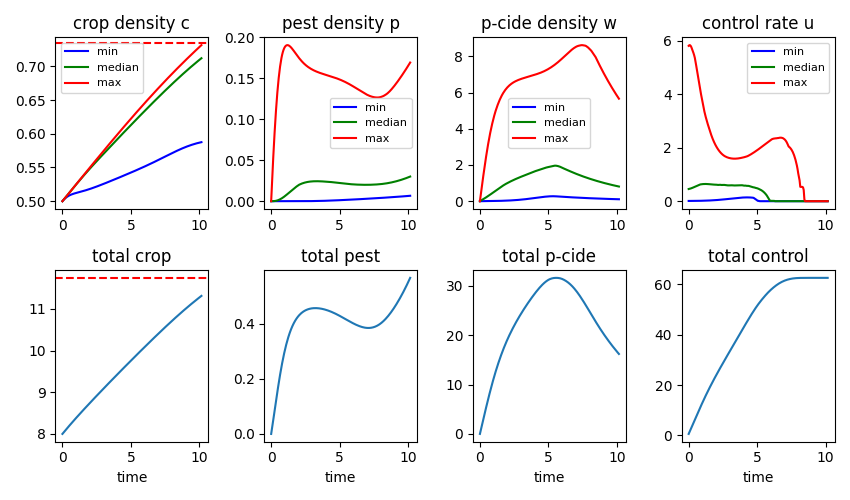
\includegraphics[width=0.8\linewidth]{../resim_240718-033400/time.png}
		\captionof{figure}{Pest attack scenario with spot spraying control. In the top row, min, median and max curves capture spatial variability. Slow pest diffusion: $d_p = 0.05$. }
		\label{fig: spotslow}
	\end{center}
\end{minipage}

\begin{minipage}{\textwidth}
	\begin{center}
		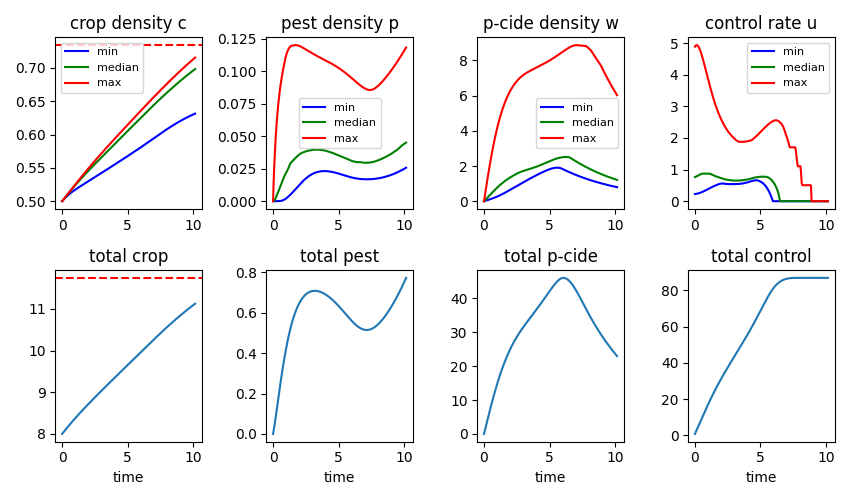
\includegraphics[width=0.8\linewidth]{../resim_240718-012904/time.png}
		\captionof{figure}{Pest attack scenario with spot spraying control. In the top row, min, median and max curves capture spatial variability. Fast pest diffusion: $d_p = 0.4$. }
		\label{fig: spotfast}
	\end{center}
\end{minipage}

\subsection{Aerial vs Spot application of pesticides}

Collecting the results for Exp 1 and Exp 2 at harvest time, we have:

\begin{center}
	\begin{tabular}{ | c | c | c| c| c| c| c| }
	\hline
	\multicolumn{7}{|c|}{Raw harvest-time totals} \\
	\hline
    method & $d_p$ & crop & pest & p-cide & cumulative control & savings \\
    \hline
    aerial & 0.05 & 11.22 & 0.63 & 32.56 & 114.85 & - \\
    \hline
    spot & 0.05 & 11.31 & 0.57 & 16.19 & 62.58 & 45.5\% \\
    \hline
    aerial & 0.4 & 11.03 & 0.85 & 29.52 & 106.24 & - \\
    \hline
    spot & 0.4 & 11.12 & 0.77 & 22.98 & 86.97 & 18.1\% \\
    \hline
    \end{tabular}
\end{center}

\begin{center}
	\begin{tabular}{ | c | c | c| c| c| c| c| }
	\hline
	\multicolumn{7}{|c|}{Crop yield normalized harvest-time totals} \\
	\hline
    method & $d_p$ & crop & pest & p-cide & cumulative control & savings \\
    \hline
    aerial & 0.05 & 1.00 & 0.06 & 2.90 & 10.24 & - \\
    \hline
    spot & 0.05 & 1.00 & 0.05 & 1.43 & 5.53 & 46.0\% \\
    \hline
    aerial & 0.4 & 1.00 & 0.08 & 2.68 & 9.63 & - \\
    \hline
    spot & 0.4 & 1.00 & 0.07 & 2.07 & 7.82 & 18.8\% \\
    \hline
    \end{tabular}
\end{center}

For the same crop yield in this scenario, optimal spot application can save $18.8\%$ to $46.0\%$ in pesticide applied over aerial spraying. Harvest quality, in terms of active pesticide on the crops, is also significantly better in spot spraying. Pests with more mobility (higher $d_p$ ) rapidly decrease the spot spraying advantage. Note is is possible that our selection of quadratic losses is favoring aerial spraying (see the conclusions section).

\section{Conclusions and Future Work}

Optimal control is capable of computing optimal spatio-temporal pesticide application strategies which could achieve large savings in pesticides for the same crop yield and quality of harvested crop. Solving the optimal control problem in 2D and time is a challenge for the implementation of Sequential Convex Programming applied here. It would be interesting to understand the limits of SCP for this PDE, and explore other solution techniques.

The optimal controls obtained via SCP appear to have some unexpected control patterns in time - utlizing pulses of control activity. Are there also some subtle control patterns occurring spatially? Further investigation of the parameter space is warranted to investigate this. In order to apply these controls to actual crop management, we would also need to integrate the detection of pest infestations into our control strategy - unless pest attack patterns were quite repeatable!

We also have not investigated various control constraints, like limits on pesticide application rate and timings. Presumably aerial control is not done continuously!

Comparing results for two different optimal control scenarios can be problematic. In our case, we are using the same cost function for two control scenarios which can have different optimal spatio-temporal behavior. One wonders, for example, if the quadratic cost disfavors the spot spraying approach, which can take advantage of large local departures from the target behavior; the quadratic cost function will selectively penalize larger departures. This argues for a Linear Programming approach, but attempts at this with \texttt{JAX/CVXPY} indicated \textit{much} slower convergence. This has not yet been attempted with the \texttt{MOSEK} solver.

Even though this method can reduce pesticide usage for some pest attack scenarios, more ecologically sound practices would rely on more subtle and natural methods of pest control. It would be interesting to investigate these techniques (e.g., EBPM \cite{R3}) in terms of optimal control. These methods can rely on the spatial relationships between parts of the managed ecosystem, and so may argue for optimization via spatio-temporal optimal control. At a minimum, more complex dynamics models would be needed; EBPM depends on establishing a more complex ecosystem to maintain the harvest compromise. 

% ----------

%\bibliography{refs}
%\bibliographystyle{plain}

\begin{thebibliography}{1}
\bibitem{R1} Ihza Rizkia Fitri, Faruda Hanum, Ali Kusnanto, Toni Bakhtiar, \textbf{Optimal Pest Control Strategies with Cost-effectiveness Analysis}, \textit{The Scientific World Journal, Hindawi Publishing Corporation}, 21 April 2021.
\bibitem{R2} Fernando Lobo Pereira, Fernando Arménio Fontes, Maria Margarida Ferreira, 
Maria do Rosário Pinho, Vilma Alves Oliveira, Eduardo Costa, and Geraldo Nunes Silva, \textbf{Conference Paper: An Optimal Control Framework for Resources Management in Agriculture}, \textit{Hindawi Publishing Corporation, Conference Papers in Mathematics},  14 July 2013.
\bibitem{R3} Miguel A. Altieri, Clara I. Nichols, and Marlene A. Fritz, 
\textbf{Manage Insects on Your Farm: A Guide to Ecological Strategies},
\textit{Sustainable Agriculture Research and Education (SARE)}, 2005.
\bibitem{R4} National Pesticide Information Center, \textbf{http://npic.orst.edu/factsheets/half-life.html}
\bibitem{R5} Stefan Bilbao,
\textbf{Numerical Sound Synthesis: Finite Difference Schemes and Simulation in Musical Acoustics, Chapter 10},
\textit{Wiley}, 2009.
\bibitem{R6} Geovani N. Grapiglia and Gabriel F. D. Stella, \textbf{An adaptive trust‑region method without function evaluations}, \textit{Computational Optimization and Applications},  82:31–60, 2022.
\bibitem{R7} Fadi Hamad and Oliver Hinder, \textbf{Conference Paper: A consistently adaptive trust-region method}, \textit{36th Conference on Neural Information Processing Systems (NeurIPS 2022)}.
\bibitem{R8} Danny C Sorensen. \textbf{Newton’s method with a model trust region modification}, \textit{SIAM Journal on
Numerical Analysis}, 19(2):409–426, 1982.
\end{thebibliography}


\section{Appendix 1: spatial control}

Plots of spatial patterns for each of the experiments are here to save space at the beginning of the document.

\subsection{Exp 1: Aerial Spraying}

Below are plots of control and state spaces at a sequence of times during the growing season. $t=10.0$ is harvest time. These plots are somewhat misleading in that the center of the spatial grid points at the boundary are really at the very edge of the field. This discrepancy is handled in cell areas in various parts of the code, but were not corrected for here. These solutions are for a $16 \times 16$ spatial grid (see Appendix 2).

\begin{minipage}{\textwidth}
	\begin{center}
		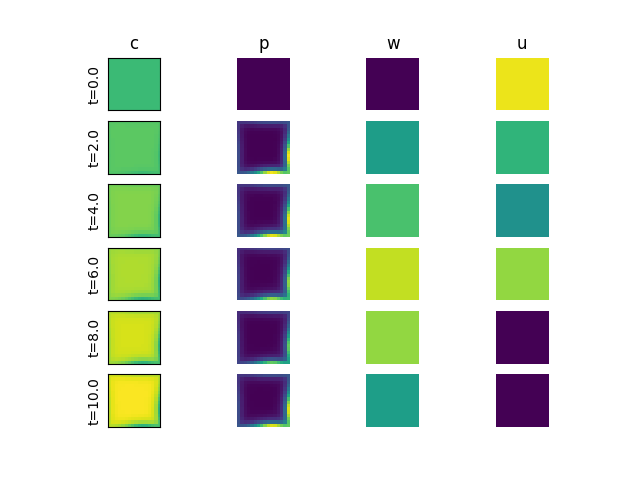
\includegraphics[width=0.8\linewidth]{../resim_240718-021040/slices.png}
		\captionof{figure}{Pest attack scenario with aerial spraying control: spatial slices.  c= crop density, p = pest density, w = pesticide density, u = pesticide application rate. Slow pest diffusion: $d_p = 0.05$.}
		\vspace{5pt}
	\end{center}
\end{minipage}

\begin{minipage}{\textwidth}
	\begin{center}
		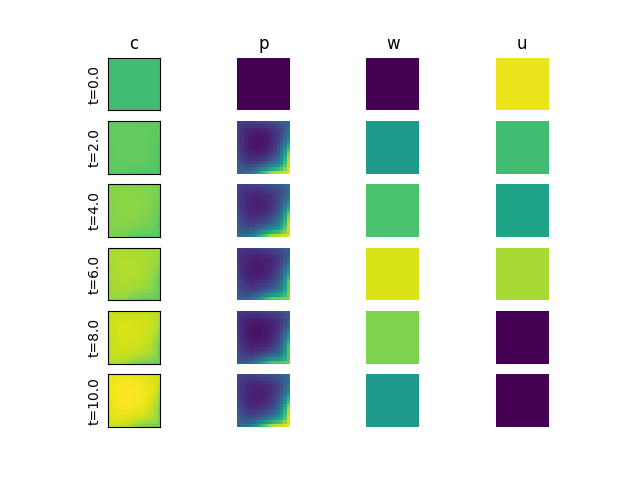
\includegraphics[width=0.8\linewidth]{../resim_240718-005456/slices.png}
		\captionof{figure}{Pest attack scenario with aerial spraying control: spatial slices.  c= crop density, p = pest density, w = pesticide density, u = pesticide application rate. Fast pest diffusion: $d_p = 0.4$.}
		\vspace{5pt}
	\end{center}
\end{minipage}



\subsection{Exp 2: Spot Spraying}

Below are plots of control and state spaces at a sequence of times during the growing season. $t=10.0$ is harvest time. These plots are somewhat misleading in that the center of the spatial grid points at the boundary are really at the very edge of the field. This discrepancy is handled in cell areas in various parts of the code, but were not corrected for here. These solutions are for a $16 \times 16$ spatial grid (see Appendix 2).

\begin{minipage}{\textwidth}
	\begin{center}
		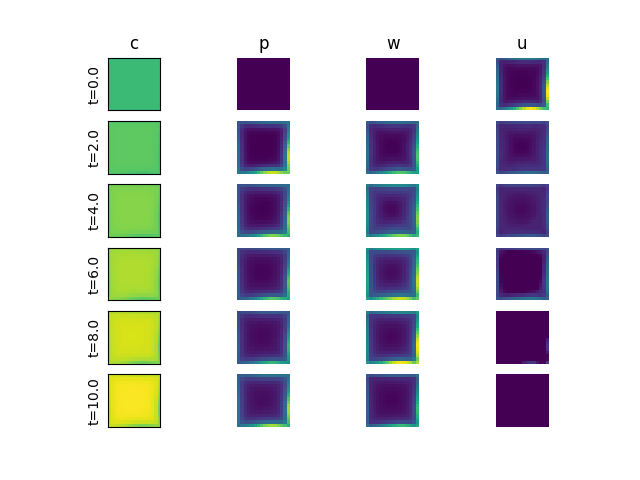
\includegraphics[width=0.8\linewidth]{../resim_240718-033400/slices.png}
		\captionof{figure}{Pest attack scenario with spot spraying control: spatial slices. c= crop density, p = pest density, w = pesticide density, u = pesticide application rate. Slow pest diffusion: $d_p = 0.05$.}
		\vspace{5pt}
	\end{center}
\end{minipage}

\begin{minipage}{\textwidth}
	\begin{center}
		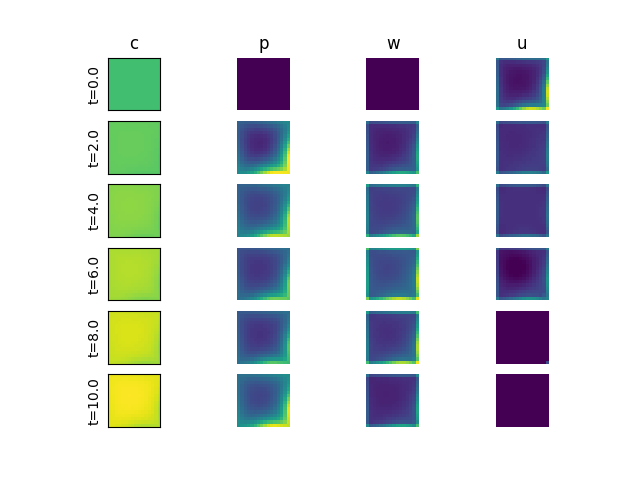
\includegraphics[width=0.8\linewidth]{../resim_240718-012904/slices.png}
		\captionof{figure}{Pest attack scenario with spot spraying control: spatial slices. c= crop density, p = pest density, w = pesticide density, u = pesticide application rate. Fast pest diffusion: $d_p = 0.4$.}
		\vspace{5pt}
	\end{center}
\end{minipage}

\section{Appendix 2: SCP convergence}

As discussed previously, an outer loop is implemented which refines the grid at the previous iteration of SCP by spatial interpolation of the control estimate. The convergence of the method is tracked in various ways and shown in the diagnostic plots below. To summarize the convergence as $n$ is refined, the following table shows the fractional change in the objective from one refinement level to the next. The first value is quite large because most of the solution refinement occurs at the low spatial resolution, where it is much faster!

As we might expect from the discussion above, we are usually below or near $5\%$ change in the relative error in the objective at $n=16$. We do not go past $n=16$ with the compute resources utilized here for time and memory reasons. More capable cloud resources (e.g., AWS) would be interesting to try.

\begin{center}
	\begin{tabular}{ | c | c | c | c | c | c | }
	\hline
	\multicolumn{6}{|c|}{Relative error convergence summary} \\
	\hline
    method & $d_p$ & $n=8$ & $n=12$ & $n=16$ & total run time (secs)\\
    \hline
    aerial & 0.05 & 33.4039 & 0.1283 & 0.0646 & 2287 \\
    \hline
    spot & 0.05 & 60.0308 & 0.0664 & 0.0374 & 4982 \\
    \hline
    aerial & 0.4 & 38.0939 & 0.1120 & 0.0480 & 3049 \\
    \hline
    spot & 0.4 & 50.0664 & 0.0990 & 0.0484 & 2029 \\
    \hline
    \end{tabular}
\end{center}

The values in this table are collected from the \texttt{outer\_ref\_error.txt} files in the relevant run directories. Run times are produced by \texttt{test\_control/test\_collect\_run\_times()}.

The detailed convergence plots in the next 2 sections show the SCP convergence over 3 values of grid refinement, $ n = \{8, 12, 16\}$. The SCP objective relative change terminates near $5\%$. The "SCP error ratio" is equivalent to $r$ in the discussion of SCP convergence in the Approach section above. Values of the SCP error ratio above the red dashed line ($\eta_1$) result in acceptance of the SCP iteration result, but values below the red dashed line results in a contraction of the SCP trust region ($\rho$). Rarely, a value of the SCP error ration above the green line ($\eta_2$) will result in an expansion of the trust region. Note that the first iteration at each grid refinement has no SCP solve as a reference, and so vales are missing for those iterations. Generally speaking, the bulk of iterations are at $n=8$, and the trust region is contracted at later iterations, although there are some curious departures from this.

\subsection{Exp 1: Aerial Spraying}

\begin{minipage}{\textwidth}
	\begin{center}
		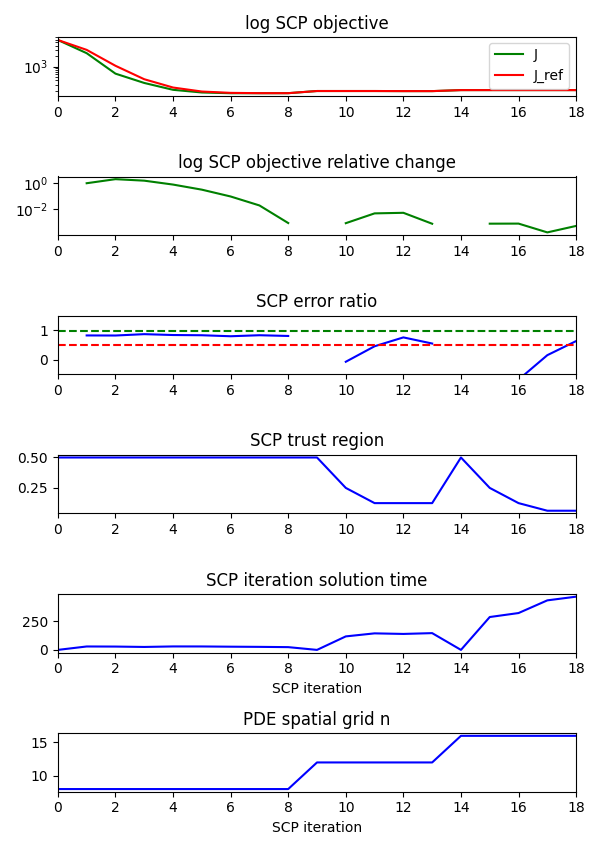
\includegraphics[width=0.8\linewidth]{../scp_240718-021040/scp.png}
		\captionof{figure}{SCP convergence. See text for details. SCP iteration solution time is in seconds. Slow pest diffusion: $d_p = 0.05$. Aerial spraying.}
		\vspace{5pt}
	\end{center}
\end{minipage}

\begin{minipage}{\textwidth}
	\begin{center}
		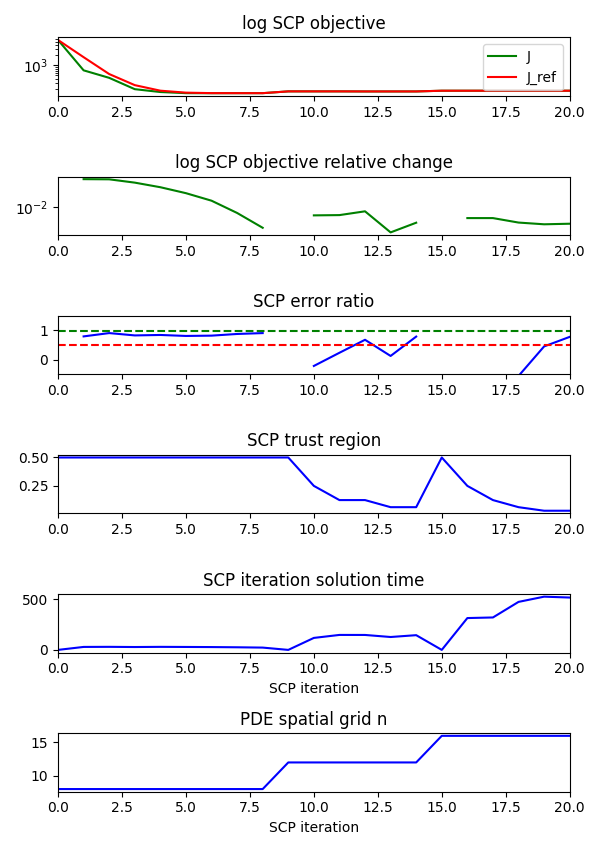
\includegraphics[width=0.8\linewidth]{../scp_240718-005456/scp.png}
		\captionof{figure}{SCP convergence. See text for details. SCP iteration solution time is in seconds. Fast pest diffusion: $d_p = 0.4$. Aerial spraying.}
		\vspace{5pt}
	\end{center}
\end{minipage}


\subsection{Exp 2: Spot Spraying}

\begin{minipage}{\textwidth}
	\begin{center}
		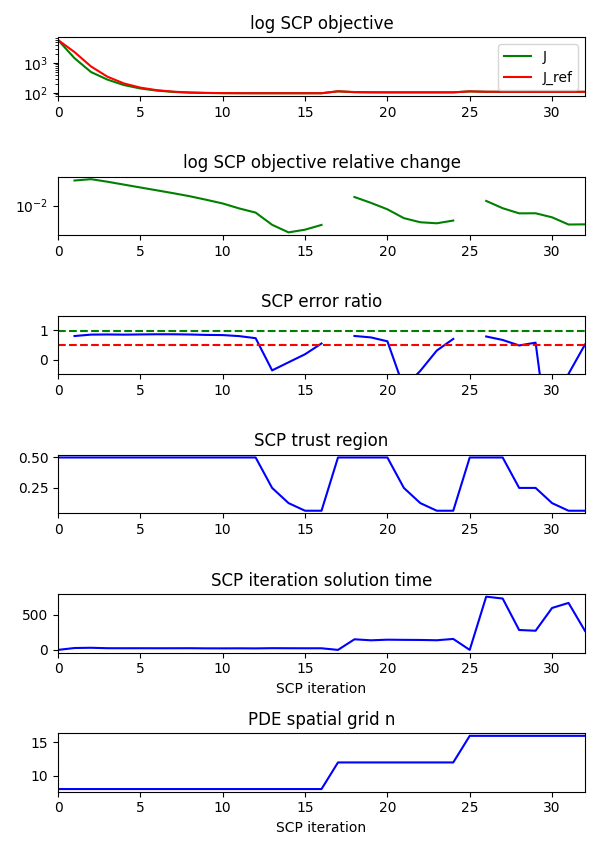
\includegraphics[width=0.8\linewidth]{../scp_240718-033400/scp.png}
		\captionof{figure}{SCP convergence. See text for details. SCP iteration solution time is in seconds. Slow pest diffusion: $d_p = 0.05$. Spot spraying.}
		\vspace{5pt}
	\end{center}
\end{minipage}

\begin{minipage}{\textwidth}
	\begin{center}
		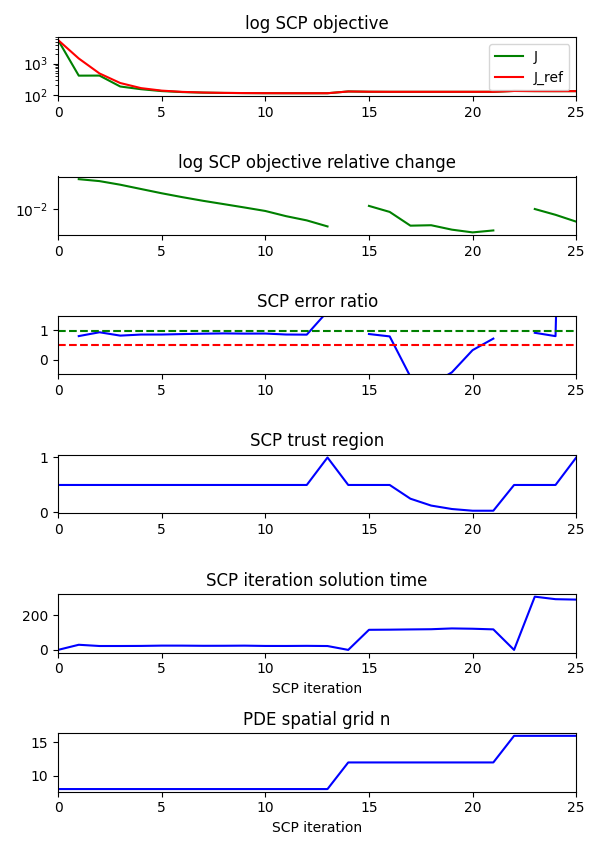
\includegraphics[width=0.8\linewidth]{../scp_240718-012904/scp.png}
		\captionof{figure}{SCP convergence. See text for details. SCP iteration solution time is in seconds.. Fast pest diffusion: $d_p = 0.4$. Spot spraying.}
		\vspace{5pt}
	\end{center}
\end{minipage}


\section{Code}

See the public github repo: \href{https://github.com/StuartGJohnson/AA203\_project}{https://github.com/StuartGJohnson/AA203\_project}.

\end{document}
